%% presentation.tex
%%
%% Presentation of the course ``Developers and their motivations'' of 
%% the Official Master on Libre Software (URJC)
%% http://master.libresoft.es
%%

%%---------------------------------------------------------------------
%%---------------------------------------------------------------------

\begin{frame}
\frametitle{¿Qué tiene de especial Wikipedia?}

\Large{``El problema con Wikipedia es que sólo funciona en la práctica.
En teoría nunca podría funcionar.''}

\bigskip
\small{Mikka Ryokas, citado por el NY Times}

\end{frame}

%%---------------------------------------------------------------------
%%---------------------------------------------------------------------

\section{¿Quién edita Wikipedia?}

%%---------------------------------------------------------------------

\begin{frame}
\frametitle{Wikipedistas}

\large{\textbf{Wikimania 2010 (Gdańsk, Polonia, julio 2010)}}

\begin{figure}[htp]
\centering
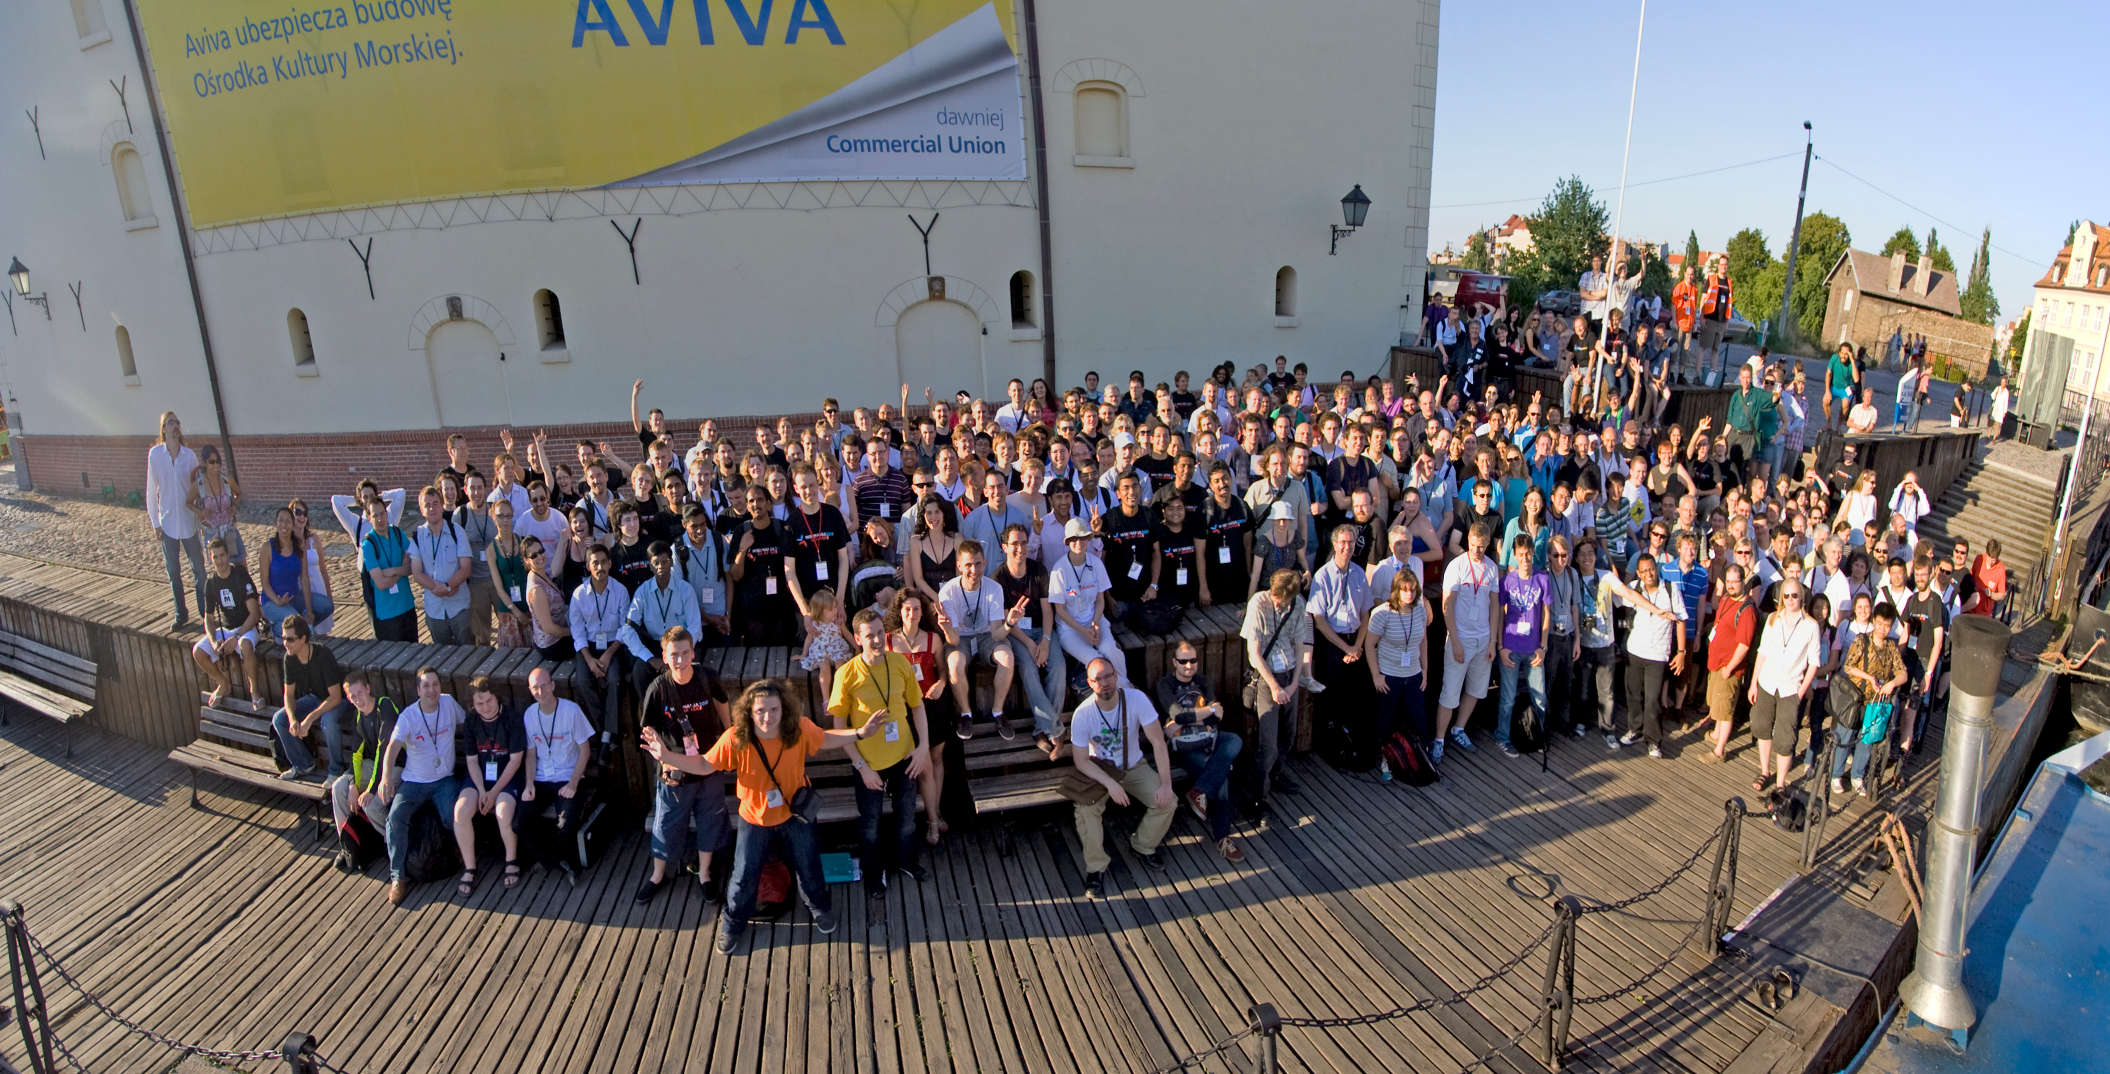
\includegraphics[width=11cm]{figs/wikimania-gdansk-2010.jpg}
% \caption{Página de usuario de Yonderboy.}
\end{figure}

\end{frame}

%%---------------------------------------------------------------------

\begin{frame}
\frametitle{Encuesta general Wikipedia}

\begin{itemize}
 \item Realizada por UNU-MERIT (2008-2010)
 \item 130.576 casos recopilados (hasta abril 2009)
\end{itemize}

\large{\textbf{Actividad}}

\begin{figure}[htp]
\centering
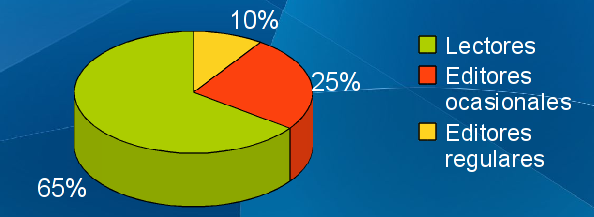
\includegraphics[width=8cm]{figs/gsurv-actividad.png}
% \caption{Página de usuario de Yonderboy.}
\end{figure}

\end{frame}

%%---------------------------------------------------------------------

\begin{frame}
\frametitle{Encuesta general Wikipedia}

\large{\textbf{Género}}

\begin{figure}[htp]
\centering
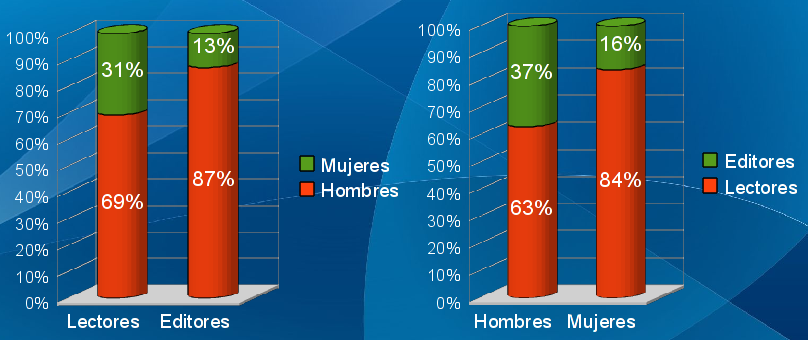
\includegraphics[width=11cm]{figs/gsurv-genero.png}
% \caption{Página de usuario de Yonderboy.}
\end{figure}

\end{frame}

%%---------------------------------------------------------------------

\begin{frame}
\frametitle{Encuesta general Wikipedia}

\large{\textbf{Estudios}}

\begin{figure}[htp]
\centering
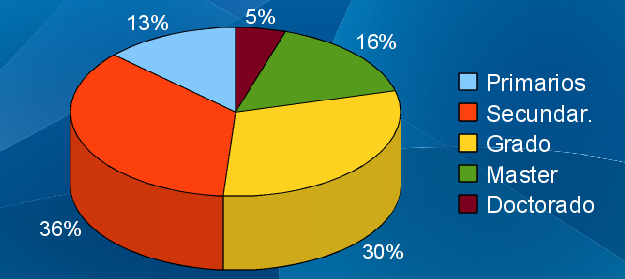
\includegraphics[width=9cm]{figs/gsurv-estudios.png}
% \caption{Página de usuario de Yonderboy.}
\end{figure}

\end{frame}

%%---------------------------------------------------------------------

\begin{frame}
\frametitle{Conclusiones del estudio}

  \begin{itemize}
   \item Razones para contribuir a Wikipedia
   \begin{itemize}
    \item ''Me gusta la idea de compartir conocimiento y quiero contribuir``
    \item ''Quería corregir un error``
    \item ''Por razones profesionales``
    \item ''La información debería estar disponible para cualquiera que desee
consultarla``
   \end{itemize}
    \item Razones para no contribuir a Wikipedia
   \begin{itemize}
    \item \alert{(25\%)}''No sé cómo contribuir``
    \item \alert{(42,2\%)}''Sería más sencillo contribuir si supiese qué áreas necesitan
mi aportación``
   \end{itemize}
   \end{itemize}
    
\end{frame}

%%---------------------------------------------------------------------
%%---------------------------------------------------------------------

\section{Evolución}

%%---------------------------------------------------------------------

\begin{frame}
\frametitle{Evolución de ediciones en artículos}

\begin{figure}[htp]
\centering
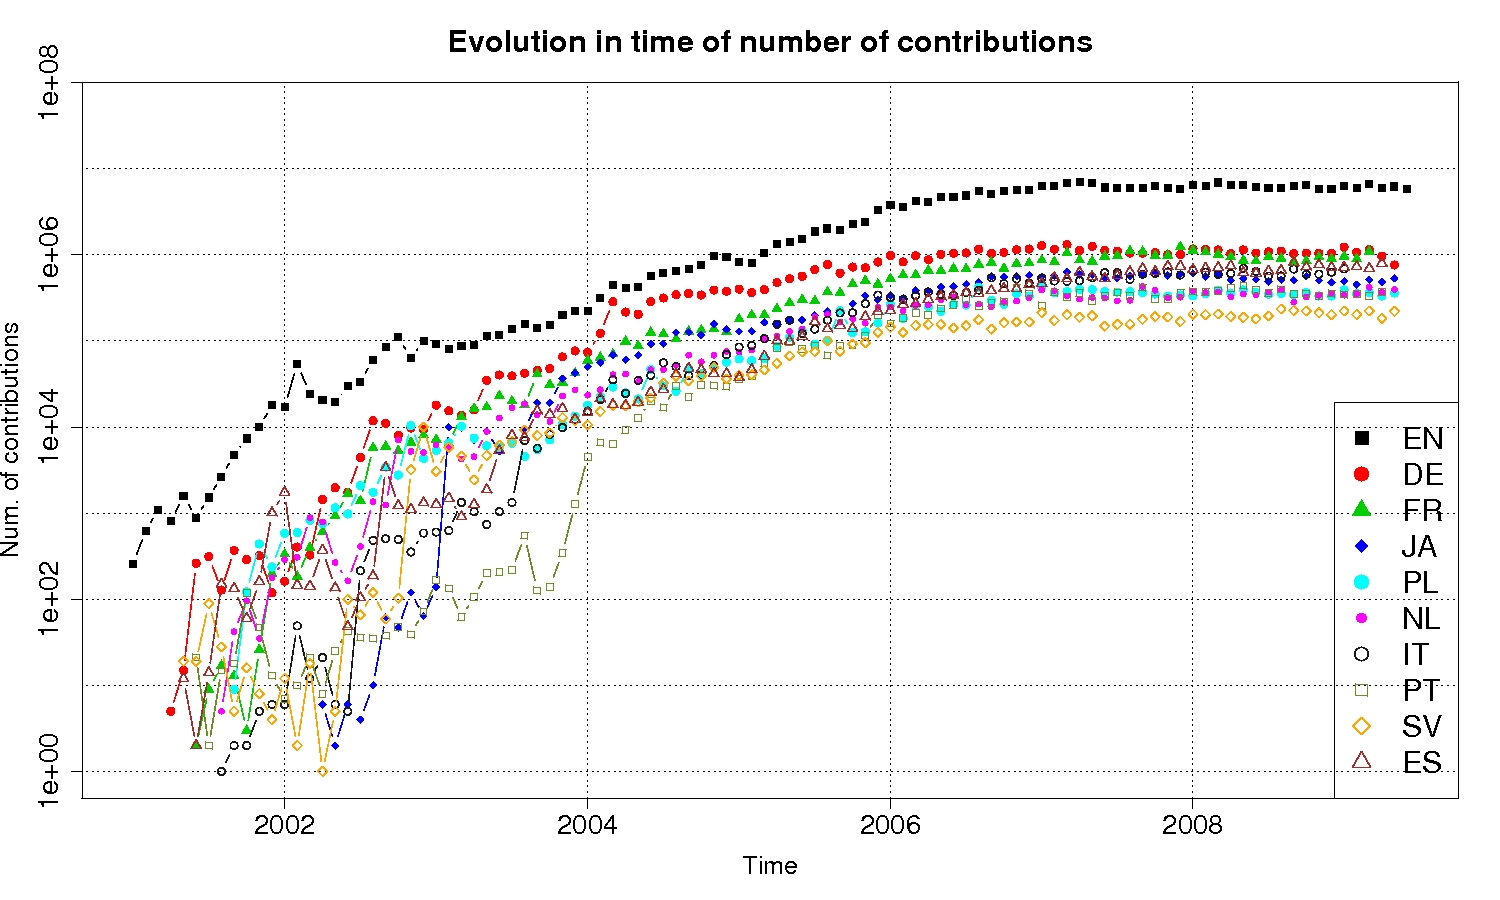
\includegraphics[width=9cm]{figs/contribs.jpg}
\end{figure}

\end{frame}

%%---------------------------------------------------------------------


\begin{frame}
\frametitle{Evolución mensual de nuevos artículos}

\begin{figure}[htp]
\centering
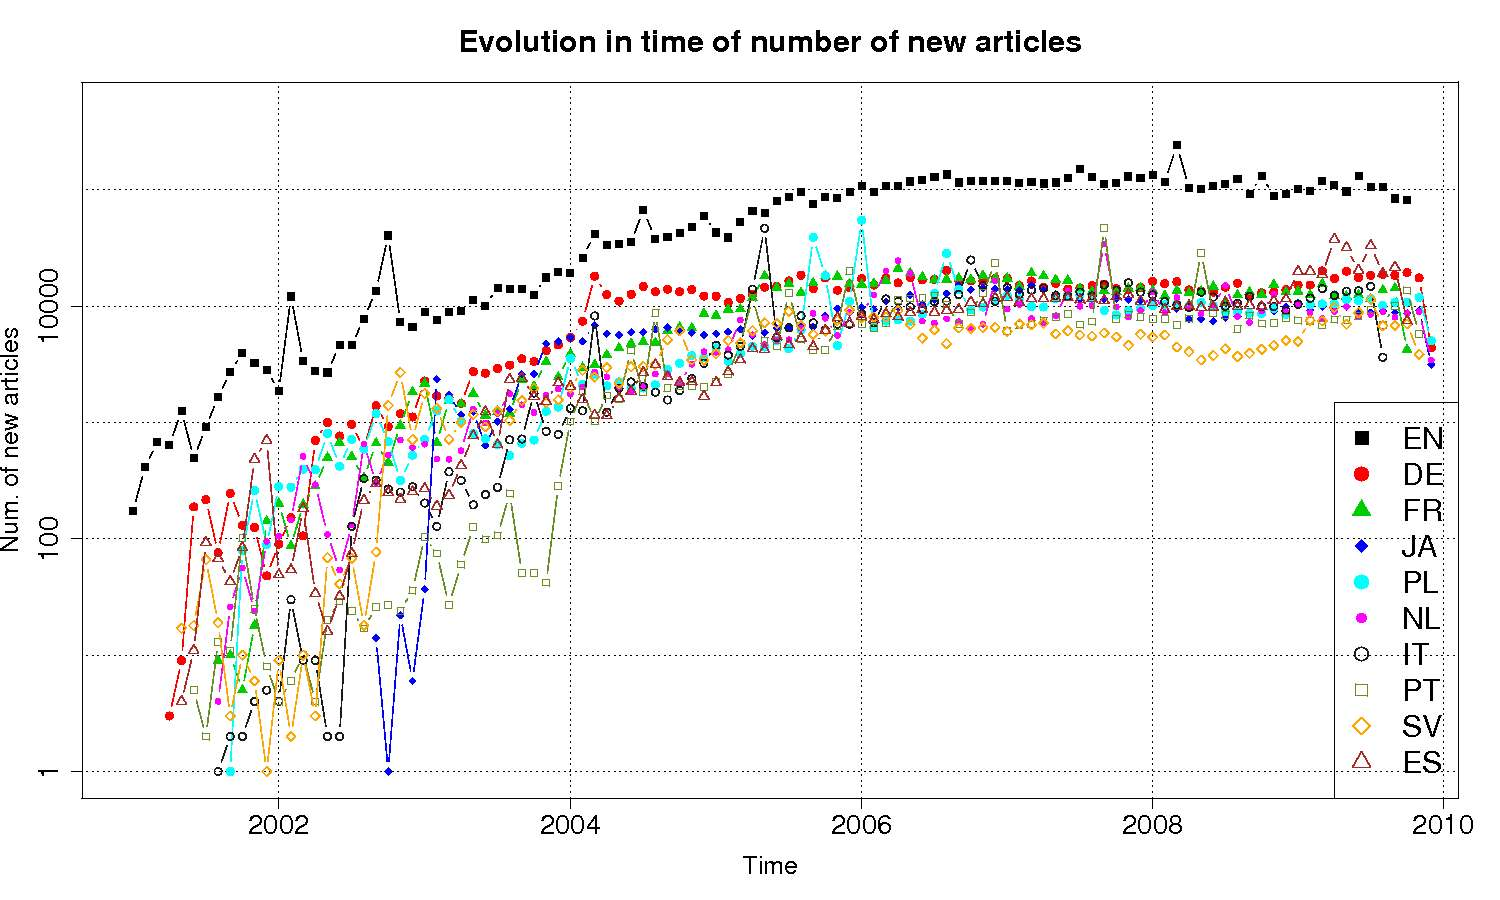
\includegraphics[width=10cm]{figs/newArticles.jpg}
% \caption{Página de usuario de Yonderboy.}
\end{figure}

\end{frame}

%%---------------------------------------------------------------------

\begin{frame}
\frametitle{Artículos más visitados}

\url{http://stats.grok.se} (Dic. 2010)

\begin{figure}[htp]
\centering
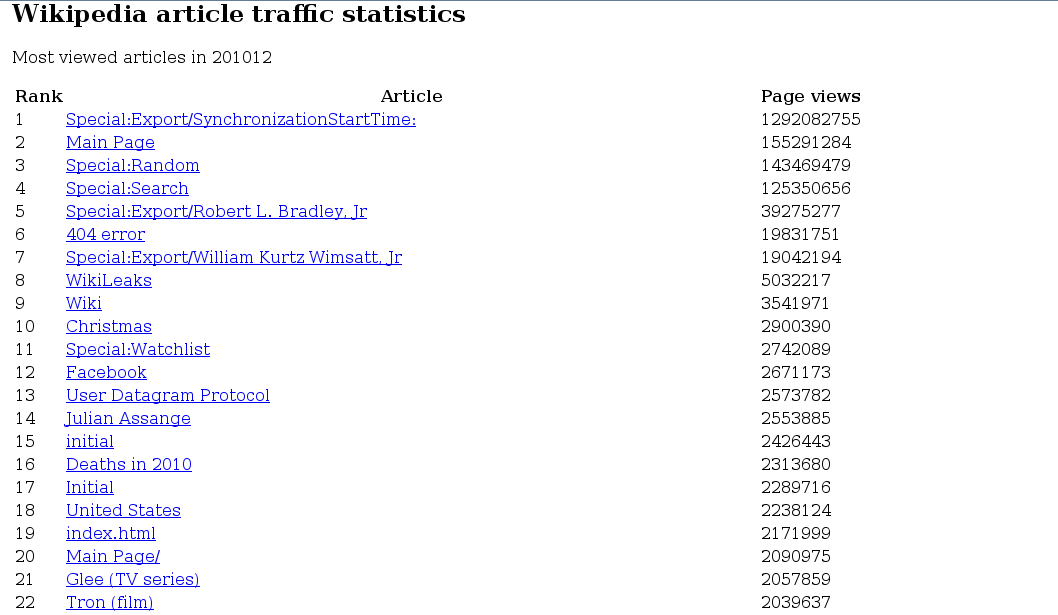
\includegraphics[width=10.75cm]{figs/wkp-traffic-dec2010.png}
\end{figure}

\end{frame}

%%---------------------------------------------------------------------

\begin{frame}
\frametitle{¿Hacen falta nuevos artículos en Wikipedia?}

\begin{itemize}
 \item Dos filosofías dentro de la comunidad de Wikipedia.
  \begin{itemize}
   \item \alert{Inclusionistas}: Propensos a mantener un artículo e intentar
mejorarlo antes que borrarlo. Argumentos:
      \begin{itemize}
       \item ''Wikipedia no es de papel``
       \item ''Es mejor tener más artículos aunque muchos no sean de gran calidad``
      \end{itemize}
   \item \alert{Deletionistas}: Apoyan la existencia de criterios precisos que deben
seguirse para admitir la creación de un nuevo artículo. Argumentos:
      \begin{itemize}
       \item Es muy costoso mejorar y ''patrullar'' un número creciente de artículos.
       \item Es mejor tener menos artículos y que muchos tengan una calidad aceptable.
       \item Suelen oponerse al uso de \textit{bots} para creación de nuevos artículos.
      \end{itemize}
  \end{itemize}

\end{itemize}

\end{frame}

%%---------------------------------------------------------------------

\begin{frame}
\frametitle{Artículos solicitados}

\texttt{http://http://es.wikipedia.org/wiki/Wikipedia:}
\texttt{Artículos\_solicitados} (Dic. 2010)

\begin{figure}[htp]
\centering
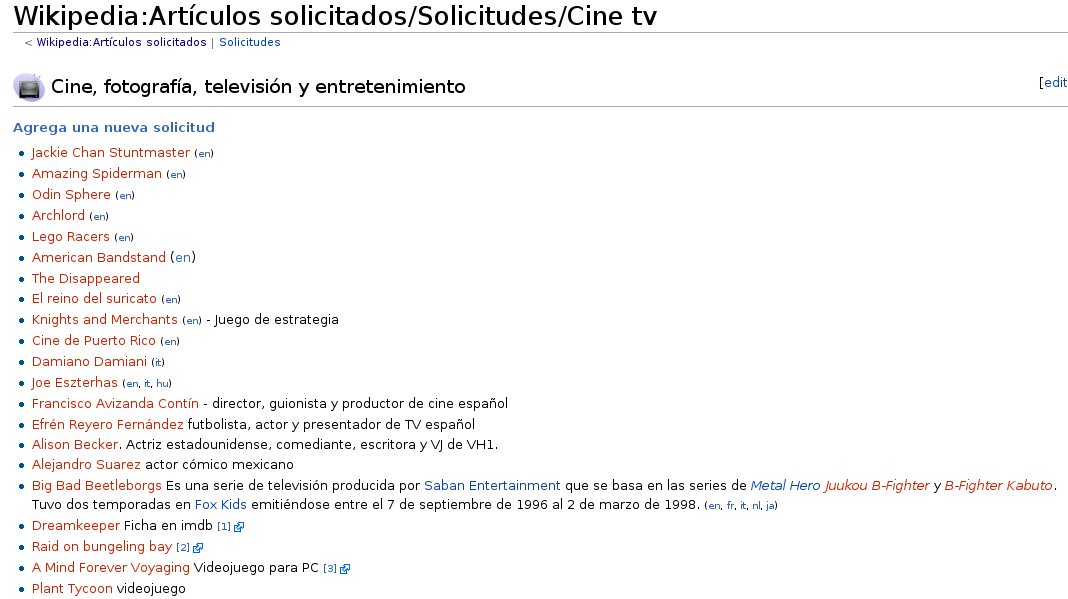
\includegraphics[width=10.5cm]{figs/articulos-solicitados-cine.png}
\end{figure}

\end{frame}

%%---------------------------------------------------------------------

\begin{frame}
\frametitle{Desigualdades en ediciones en Wikipedia}

\begin{itemize}
 \item Existe un \alert{núcleo} (aprox. un 5\% del total de editores) que concentran
la mayor parte de contribuciones en las 10 mayores Wikipedias (90\% del total
de revisiones).
 \item Valida la percepción intuitiva que Jimmy Wales expresó en una conferencia
en 2005.
  \item Si estudiamos cómo se reparten las ediciones entre los artículos la
desigualdad es menos acusada (56\%-69\%).

\end{itemize}

\end{frame}

%%---------------------------------------------------------------------

\begin{frame}
\frametitle{Evolución de las reversiones}

\bigskip
Notable incremento (x4) en reverts, excepto para usuarios experimentados.

\begin{figure}[htp]
\centering
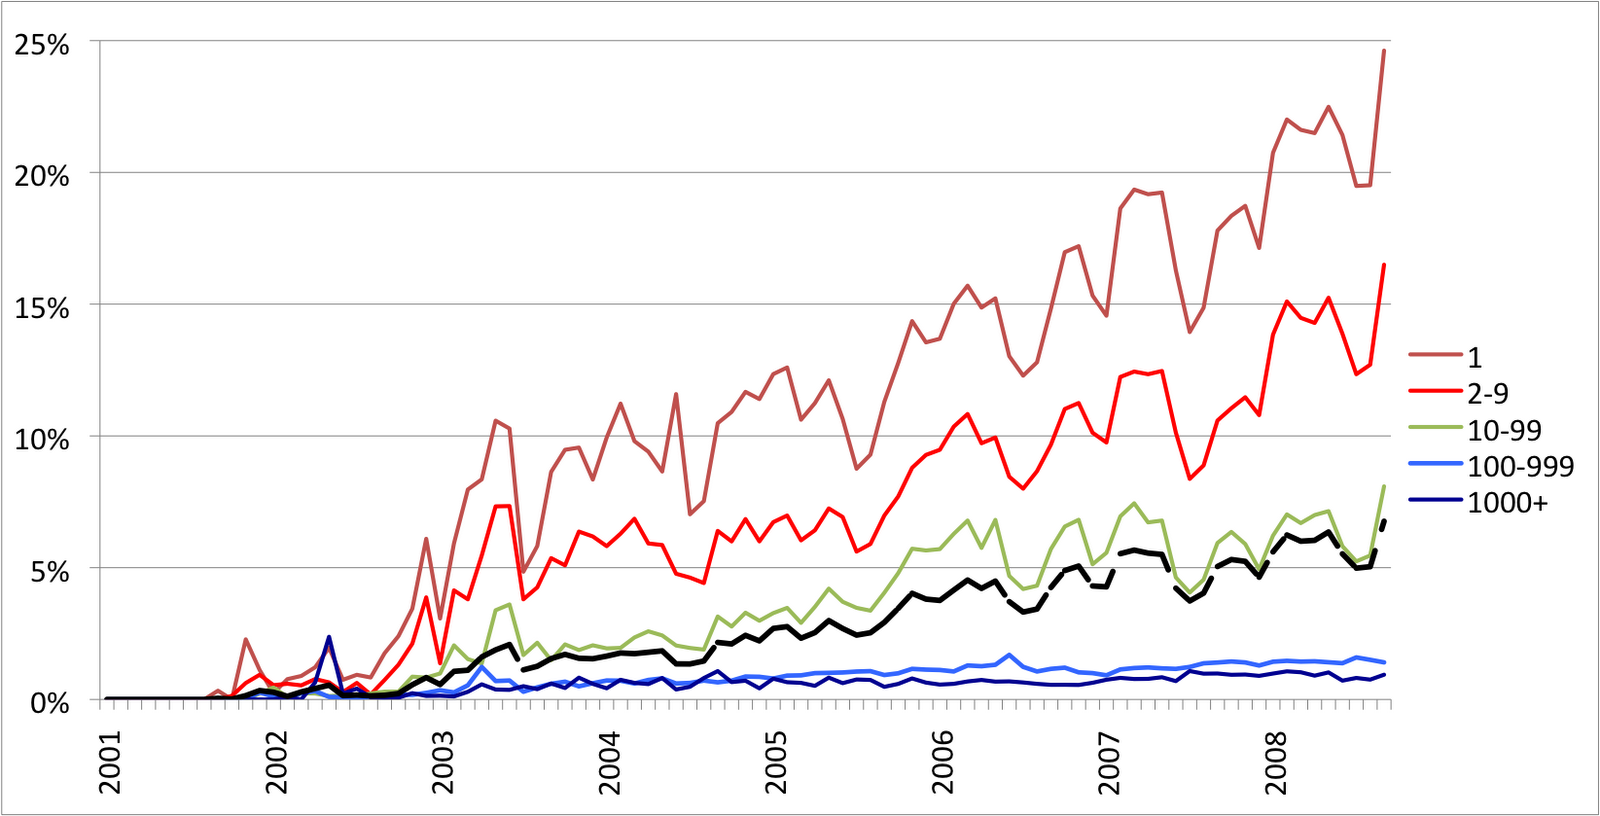
\includegraphics[width=8.5cm]{figs/reverts-evol.png}
\caption{Augmented Social Cognition Group (PARC; CA, EE.UU.)}
\end{figure}

\end{frame}

%%---------------------------------------------------------------------
%%---------------------------------------------------------------------

\section{Calidad y fiabilidad}

%%----------------------------------------------------------------------

\begin{frame}
\frametitle{¿Son fiables los artículos de Wikipedia?}

    \begin{itemize}
     \item Intuitivamente, parece que fuese imposible si todo el mundo contribuye
libremente, ya que no existiría orden ni concierto.
     \item Sin embargo, se puede llegar a crear contendio fiable (AD, artículos buenos...).
     \item La clave está en que sí existe una organización dentro de la
comunidad que permite mejorar la calidad del contendio.
    \end{itemize}

\end{frame}

%%----------------------------------------------------------------------

\begin{frame}
\frametitle{¿Son fiables los artículos de Wikipedia?}

\textbf{Pauta sensatas de uso}
    \begin{itemize}

     \item Wikipedia, como cualquier otra enciclopedia electrónica o impresa, es
una fuente \textit{terciaria} de información, por lo que no se debería citar en
trabajos académicos.

     \item Es conveniente seguir las fuentes de información citadas, verificar
las referencias y formarnos una opinión contrastada a partir de ellas, usando Wikipedia
como base para iniciar la búsqueda.

     \item \textit{Why you can't cite Wikipedia in my class} (11-2007): Departamento de Historia
de Middlebury veta las citas a cualquier enciclopedia, incluida Wikipedia.
    \end{itemize}

\end{frame}

%%----------------------------------------------------------------------

\begin{frame}
\frametitle{Hacia una Wikipedia de calidad}

\Large{La elección de Wikipedia}
\bigskip

\normalsize{Se toman medidas para intentar mitigar los vandalismos, revisar
frecuentemente el contenido de artículos y formentar su mejora, pero siempre
respetando la libertad de cualquier persona para editar}

\bigskip
\Large{\textbf{¿Es posible que en un futuro todos los artículos sean fiables?}}

\end{frame}

\begin{frame}
\frametitle{Aclarando conceptos}

  \begin{itemize}

    \item Calidad no es sinónimo de fiabilidad

    \item Además de no contener errores, hay muchos criterios adicionales
que podríamos usar para medir la \alert{calidad} de un artículo de Wikipedia.

    \begin{itemize}
     \item Estilo de redacción accesible y divulgativo.
     \item Artículo no excesivamente extenso.
     \item Buena organización de contenidos, coherencia entre secciones.
     \item Inclusión de imágenes, contenido multimedia.
     \item Abundancia de referencias y citas 
    \end{itemize}
  \end{itemize}

\end{frame}

%%----------------------------------------------------------------------

\begin{frame}
\frametitle{Asesoramiento de calidad de contenidos}

  \begin{itemize}

    \item Proyecto Wikipedia 1.0

    \item Equipo de voluntarios que revisa el contenido de los artículos
de Wikipedia, marcando un nivel de calidad orientativo.

    \begin{itemize}
     \item Artículo destacado.
     \item Artículo bueno
     \item Clases intermedias (B, C, iniciales) sólo marcados en algunas
Wikipedias.
     \item Esbozos: artículos muy cortos, en estado inicial.
    \end{itemize}
  \end{itemize}

\url{http://en.wikipedia.org/wiki/Wikipedia:Assessment}

\end{frame}

%%----------------------------------------------------------------------

\begin{frame}
\frametitle{Revisión de Artículos Destacados}

  \begin{itemize}

    \item Se sigue un riguroso proceso de revisión antes de promocionar los
artículos al máximo nivel de calidad. 

    \begin{itemize}
     \item El artículo es propuesto para su nominación como destacado.
     \item Numerosos miembros de la comunidad lo revisan.
     \item Se espera que el promotor(es) de la nominación trabaje en
colaboración con otros para mejorarlo según los comentarios.
     \item Si hay un amplio consenso, se promociona el artículo, que ya puede
aparecer en la página principal de Wikipedia.
    \end{itemize}
    \item Los AD también pueden perder su estatus si empeoran posteriormente.
  \end{itemize}

\end{frame}

%%----------------------------------------------------------------------

\begin{frame}
\frametitle{Estadísticas Wikipedia en inglés}

\begin{figure}[htp]
\centering
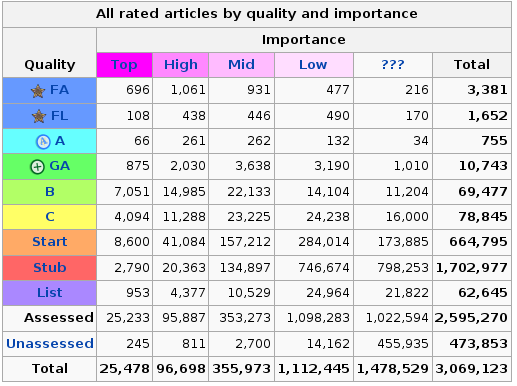
\includegraphics[width=7cm]{figs/quality-articles-stats.png}
\end{figure}

\end{frame}

%%----------------------------------------------------------------------

\begin{frame}
\frametitle{Ciclo de mejora de un artículo}

\Large{\textbf{Ciclo de vida del artículo \textit{Atom} en inglés}}

\begin{figure}[htp]
\centering
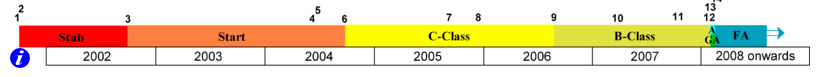
\includegraphics[width=12cm]{figs/ciclo-articulo-destacado.png}
\end{figure}

\end{frame}

%%----------------------------------------------------------------------

\begin{frame}
\frametitle{Rasgos comunes Artículos Destacados}

\begin{itemize}
 \item Hacen falta al menos 1.000 días (casi 3 años) para que un artículo se
convierta en Artículo Destacado en Wikipedia.
 \item En promedio, los artículos destacados tienen 10 veces más editores diferentes
que los artículos estándar (200 veces más en la versión inglesa).
 \item Los AD son revisados en todo caso por un número significativo de editores con
larga experiencia en el proyecto (más de 1.000 días de permanencia).
 \item Es especialmente importante mantener a estos editores para mantener la calidad
del proyecto a buen nivel.
\end{itemize}

\end{frame}

%%----------------------------------------------------------------------

\begin{frame}
\frametitle{Wikiproyectos y Wiportales}

  \begin{itemize}

    \item Algunos autores se organizan en Wikiproyectos. Son grupos 
editoriales para colaborar en artículos de temática relacionada. 

    \item Animan la colaboración entre usuarios, y la oragnización para
mejorar la calidad de los artículos de un área concreta.

    \item No hay normas estrictas sobre el tipo de tema a elegir o el tamaño
del grupo.

    \item Los Wikiportales agrupan artículos de temática relacionada. No tienen
por qué estar asociados a un Wikiproyecto, pero con frecuencia la conexión es
muy estrecha.

   \end{itemize}

\end{frame}

%----------------------------------------------------------------------

\begin{frame}
\frametitle{Ejemplo de Wikiproyecto}

\begin{figure}[htp]
\centering
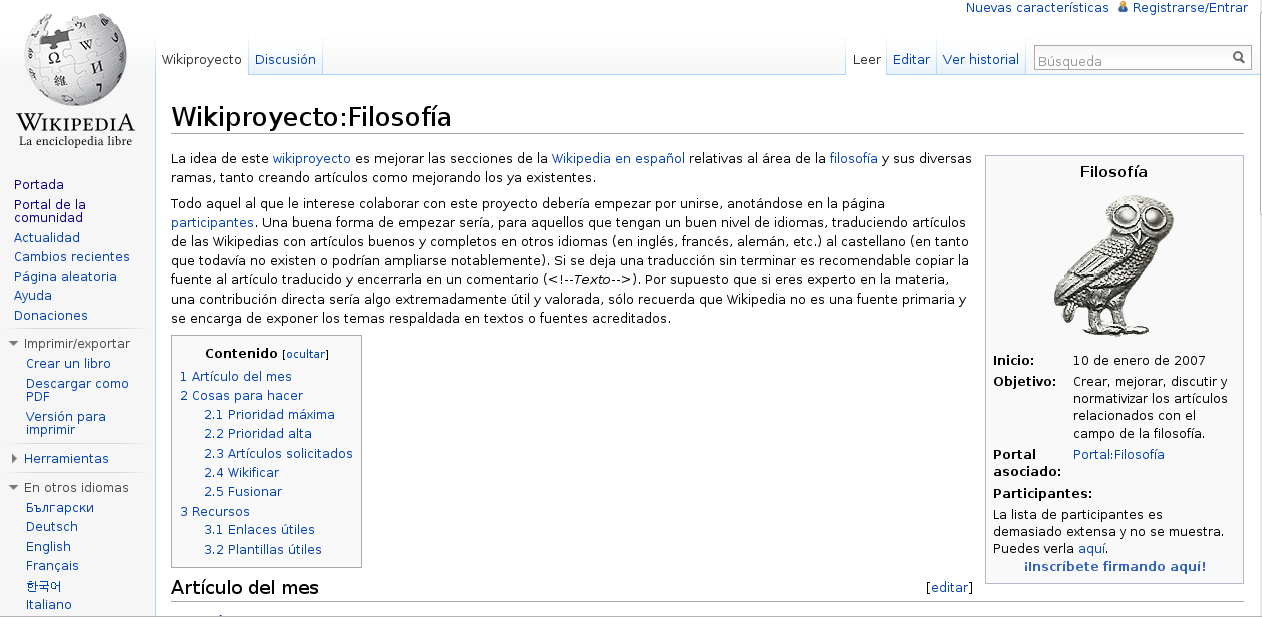
\includegraphics[width=10cm]{figs/wikiproyecto-filosofia.png}
\caption{Wikiproyecto Filosofía en la Wikipedia en español}
\end{figure}

\end{frame}

%%----------------------------------------------------------------------

\begin{frame}
\frametitle{Ejemplo de Wikiportal}

\begin{figure}[htp]
\centering
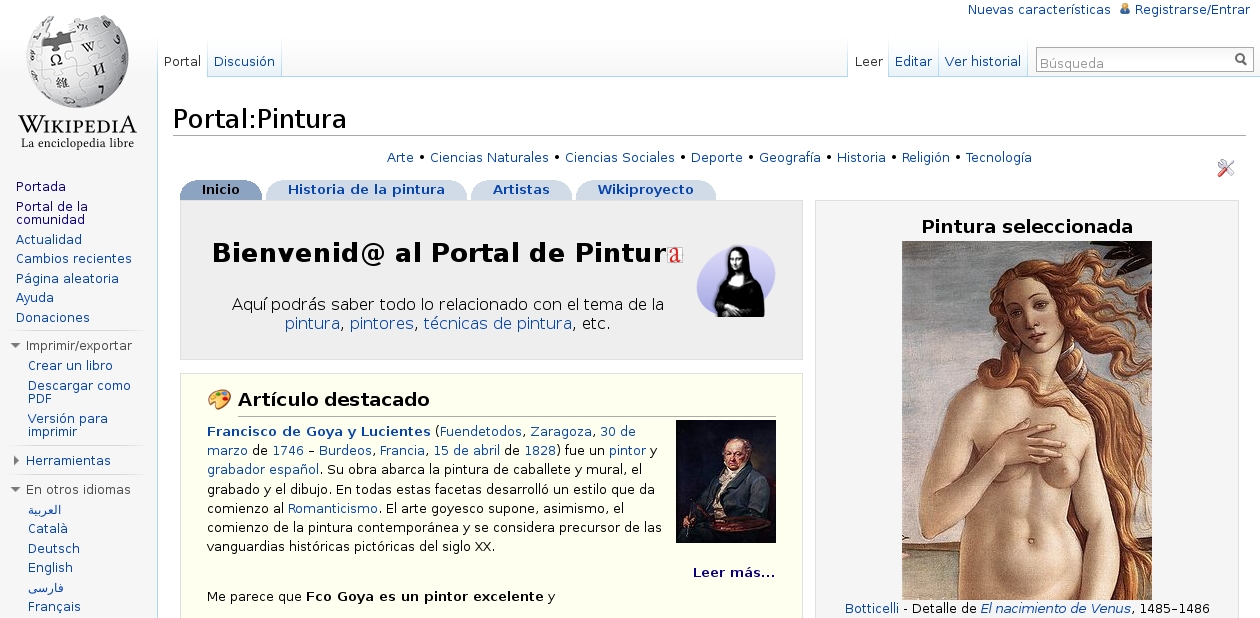
\includegraphics[width=10cm]{figs/wikiportal-pintura.png}
\caption{Wikiportal Pintura en la Wikipedia en español}
\end{figure}

\end{frame}

%%----------------------------------------------------------------------

\begin{frame}
\frametitle{Noticias y ediciones inmediatas}

    \begin{itemize}
      \item Wikipedia es capaz de recoger la información conforme va ocurriendo.

      \item Ejemplos

      \begin{itemize}
    \item Artículo del 11-S.
    \item Artículo del 11-M.
    \item Artículo del terremoto de L'Aquila.
    \item Citas periódicas: Olimpiadas, campeonatos, vueltas ciclistas...
     \item Partido de tenis más largo de la historia (Wimbledon, 06-2010).
      \end{itemize}

    \end{itemize}

\end{frame}

%%----------------------------------------------------------------------

\begin{frame}
\frametitle{Noticias y ediciones inmediatas}

    \begin{itemize}
      \item Pero también hay que tener cuidado con informaciones no
contrastadas.

      \begin{itemize}
        \item \textit{Artículo de Sinbad}. El actor fue (error) dado por muerto.
	\item \textit{John Seigenthaler Sr}. (editor retirado USA Today). Acusado
de conspiración en asesinato de JFK y Bob Kennedy (error).
	\item \textit{Senador Ted Kenedy}. Se informó (OK) que había sufrido
un infarto y (error) que había fallecido.
	\item \textit{Aimé Césaire}. Autor dominicano, se informó (OK) de su muerte días antes
de que realmente ocurriera.
	\item \textit{Andrea Dworkin}. Activista feminista y escritora. Se informó (OK)
de su muerte el mismo día, antes que cualquier medio de comunicación.
	\item \textit{Tim Russert}. Presentador en la NBC, murió en la central de la cadena en
Washington. Su muerte (OK) apareció en Wikipedia antes de que la propia cadena lo anunciara.
      \end{itemize}

    \end{itemize}

\end{frame}

%%----------------------------------------------------------------------

\begin{frame}
\frametitle{Noticias y ediciones inmediatas}

    \begin{itemize}
      \item Curiosamente, el proyecto Wikinoticias está precisamente dedicado
a labores periodísticas y de actualidad.

      \item \url{http://es.wikinews.org/wiki/Main_Page}

      \item Sin embargo, la visibilidad de Wikipedia (sobre todo en inglés)
sigue polarizando la atención de los editores. A pesar de que la información
de la enciclopedia debe ser estable y contrastada.

    \end{itemize}


\end{frame}

%%----------------------------------------------------------------------

\begin{frame}
\frametitle{Noticias y ediciones inmediatas}

    \begin{figure}[htp]
    \centering
    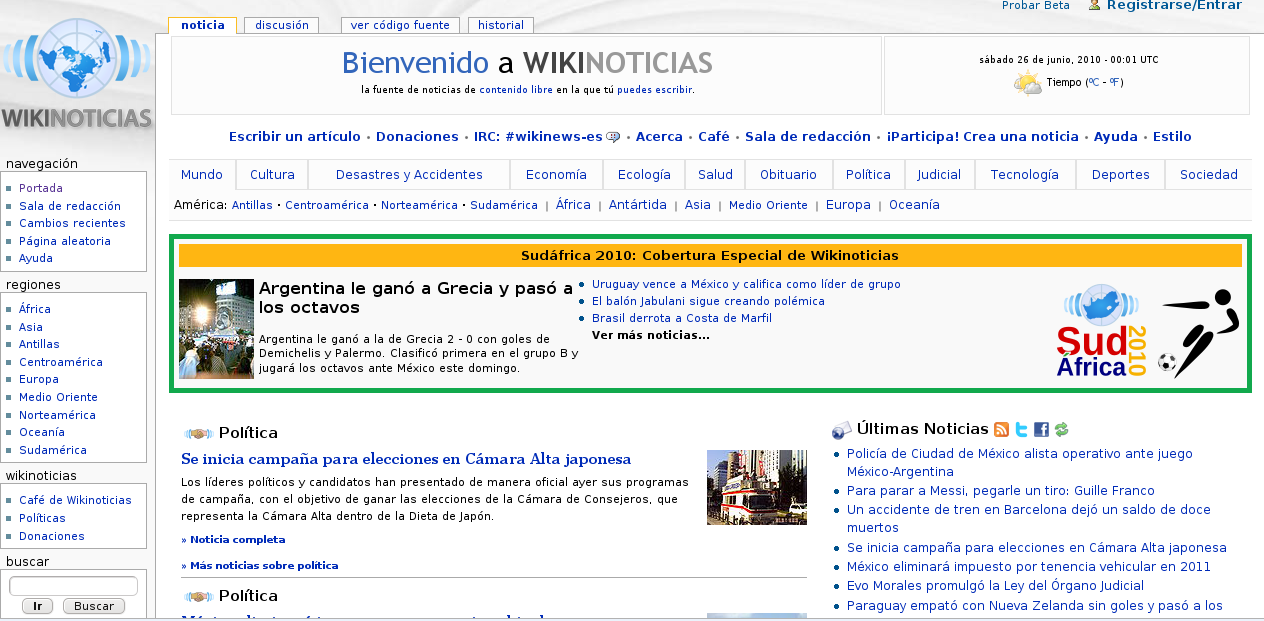
\includegraphics[width=10.5cm]{figs/wikinews.png}
    \caption{Portada del proyecto Wikinoticias}
    \end{figure}

\end{frame}

%%---------------------------------------------------------------------
%%---------------------------------------------------------------------

\section{Futuro y sostenibilidad de Wikipedia}

%%----------------------------------------------------------------------

\begin{frame}
\frametitle{Strategy Plan: prioridades}

\url{http://strategy.wikipedia.org}

    \begin{figure}[htp]
    \centering
    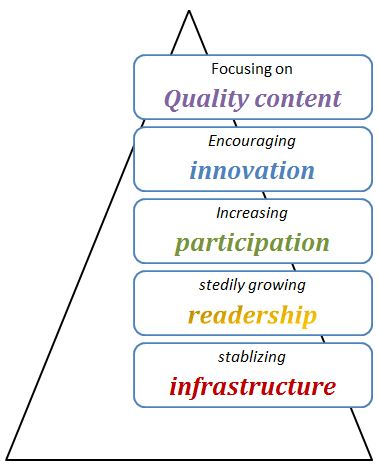
\includegraphics[width=3.5cm]{figs/Strategywiki-stability-priorities.jpg}
    \caption{Prioridades Wikipedia}
    \end{figure}

\end{frame}

%%----------------------------------------------------------------------

\begin{frame}
\frametitle{Strategy Plan: Editores activos (+5 ediciones/mes)}

\url{http://strategy.wikimedia.org/wiki/Active_contributors}

    \begin{figure}[htp]
    \centering
    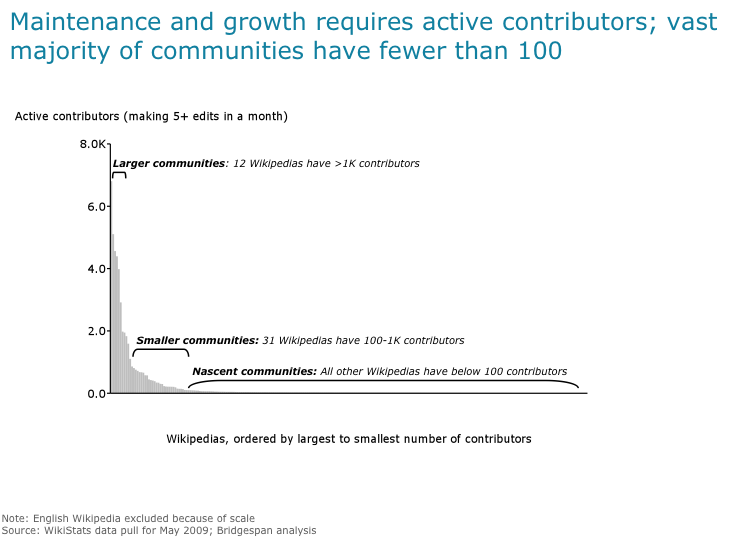
\includegraphics[width=9.5cm]{figs/Active-contributors-by-wikipedia.png}
    \caption{Distribución de Wikipedias según número de editores activos}
    \end{figure}

\end{frame}

%%----------------------------------------------------------------------

\begin{frame}
\frametitle{Strategy Plan: Evolución sostenible}

\url{http://strategy.wikimedia.org/wiki/Strategic_Plan/Movement_Priorities}

    \begin{figure}[htp]
    \centering
    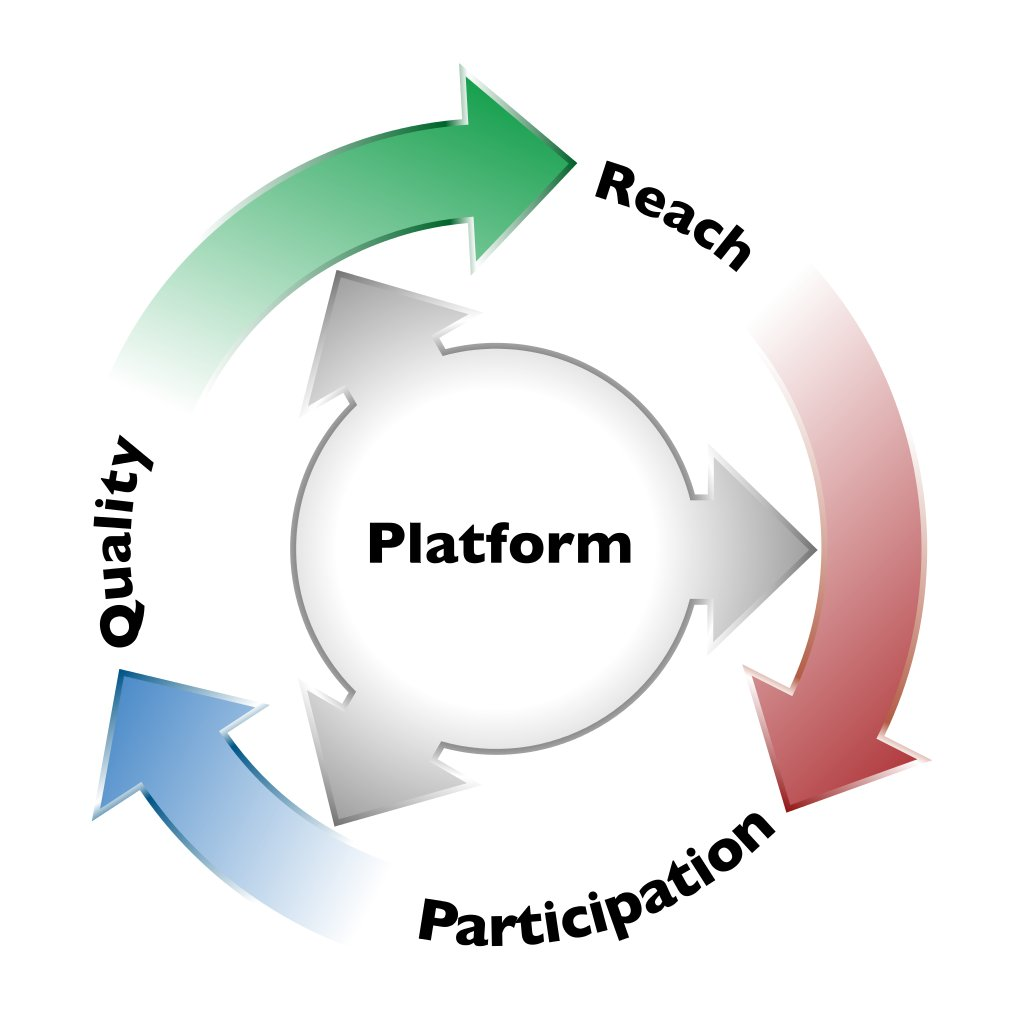
\includegraphics[width=4.5cm]{figs/Virtuous-Circle.jpg}
    \caption{Ciclo de evolución sostenible de proyectos WMF}
    \end{figure}

\end{frame}

%%----------------------------------------------------------------------

\begin{frame}
\frametitle{Strategy Plan: Prioridades de WMF}

\small{\url{http://strategy.wikimedia.org/wiki/Strategic_Plan/Role_of_the_WMF}}

    \begin{figure}[htp]
    \centering
    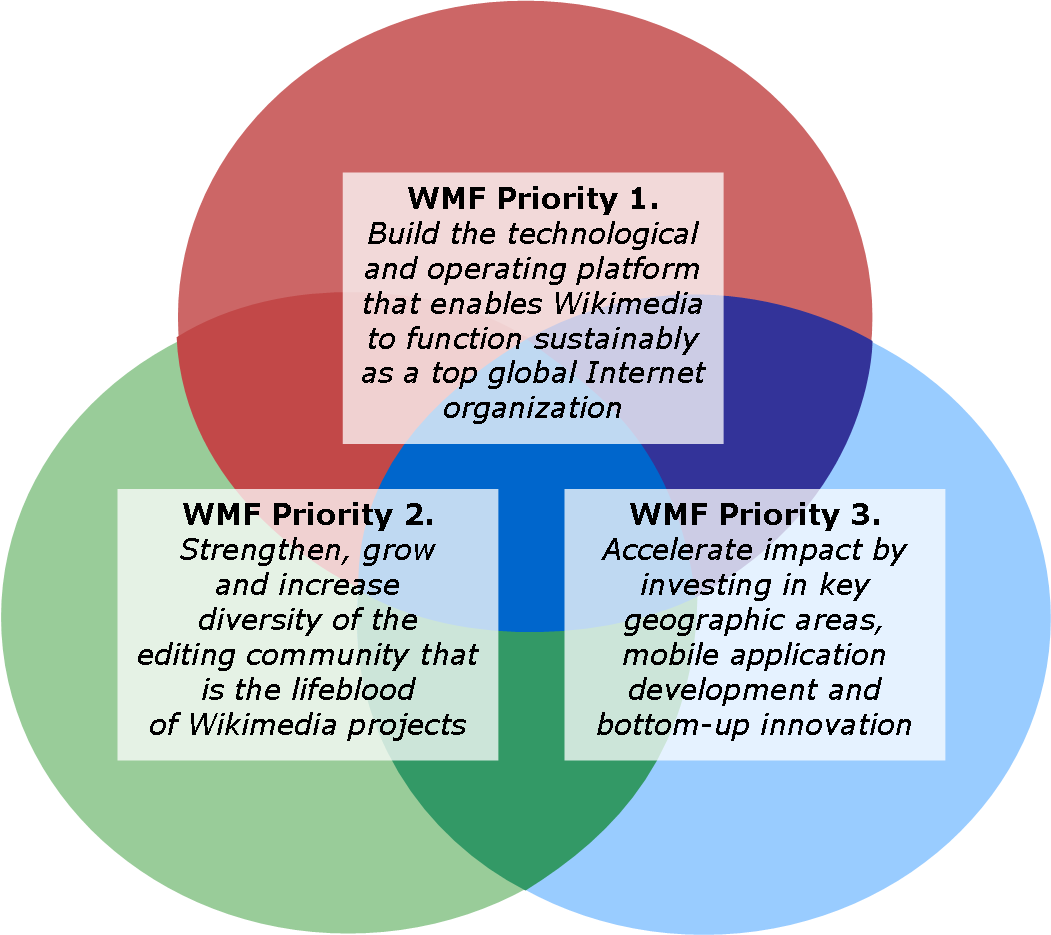
\includegraphics[width=5.5cm]{figs/WMF-Priorities.png}
    \caption{Papel de Wikimedia Foundation}
    \end{figure}

\end{frame}

%%----------------------------------------------------------------------

\begin{frame}
\frametitle{Capítulos WMF}

\url{http://strategy.wikimedia.org/wiki/Wikimedia_Chapters}

    \begin{figure}[htp]
    \centering
    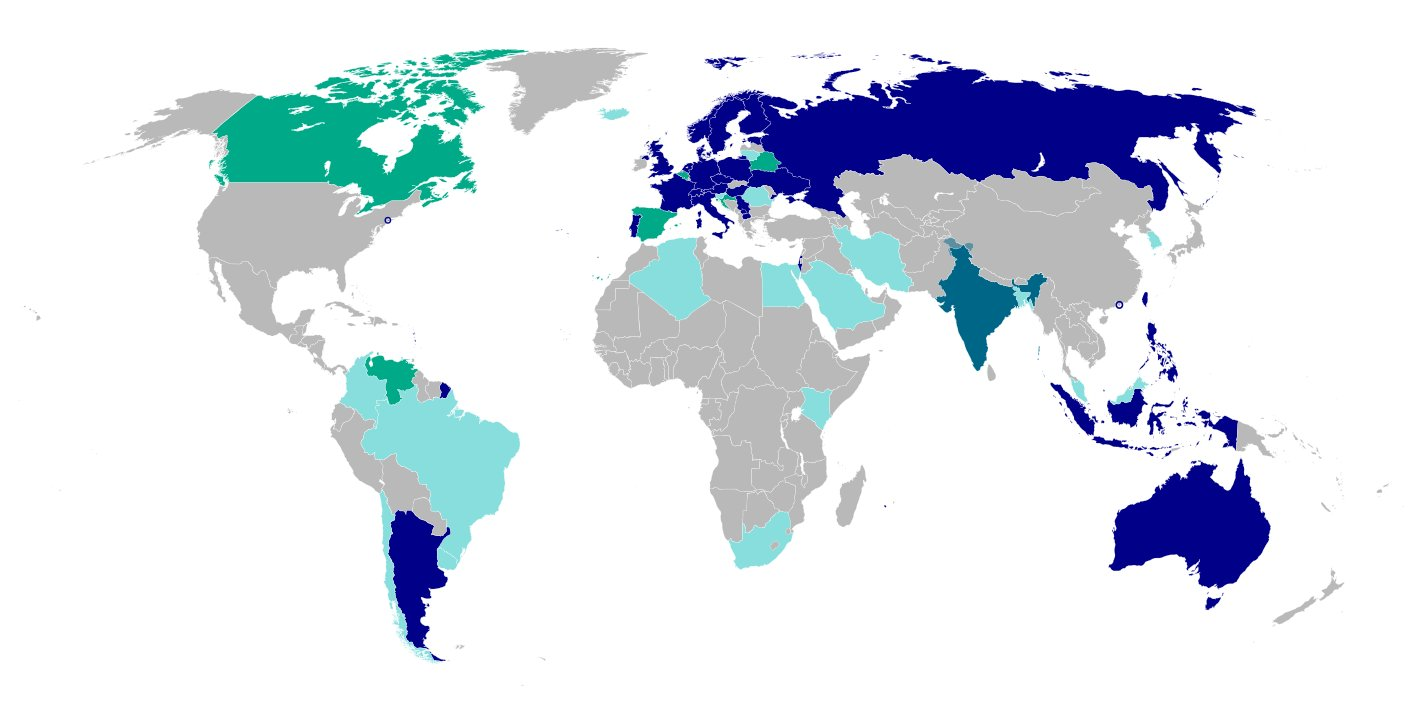
\includegraphics[width=10.5cm]{figs/Wikimedia-chapters.jpg}
    \caption{Capítulos WMF existentes y en proceso de creación}
    \end{figure}

\end{frame}

%%----------------------------------------------------------------------

\begin{frame}
\frametitle{Fiesta 10 años de Wikipedia (Madrid)}

    \begin{itemize}
      \item Auditorio Edificio Telefónica I+D.
      \item C/ Emilio Vargas, 6.
      \item Sábado 15 de enero, 12.00.
      \item Charla coloquio abierta.
      \item Personalidades del mundo de contenidos y obras culturales libres.
      \item Fiesta de celebración 10 años de Wikipedia.

      \item \url{http://es.wikinews.org/wiki/Main_Page}

      \item Sin embargo, la visibilidad de Wikipedia (sobre todo en inglés)
sigue polarizando la atención de los editores. A pesar de que la información
de la enciclopedia debe ser estable y contrastada.

    \end{itemize}


\end{frame}
